\documentclass[]{beamer}
%\documentclass{article}
%\usepackage{beamerarticle}

\mode<presentation>
{
  \usetheme{Warsaw}
  % or ...

  \setbeamercovered{transparent}
  % or whatever (possibly just delete it)
}


\usepackage[english]{babel}
% or whatever

\usepackage[utf8]{inputenc}
% or whatever

\usepackage{times}
\usepackage[T1]{fontenc}
\usepackage{tikz}
\usetikzlibrary{arrows.meta}

%%%%%%%%%%%%%%%%%%%%%%%%%%%%%%%%%%
%%                         PACKAGES                      %%
%%%%%%%%%%%%%%%%%%%%%%%%%%%%%%%%%%
\usepackage{hyperref,ctable}
\usepackage{graphicx}
\usepackage{tikz}                    % For flowchart
\usetikzlibrary{shapes,arrows} % For flowchart


%%%%%%%%%%%%%%%%%%%%%%%%%%%%%%%%%%
%%                           COLORS                        %%
%%%%%%%%%%%%%%%%%%%%%%%%%%%%%%%%%%
%AU COLORS
\definecolor{aublue}{RGB}{25,33,129}
\definecolor{aured}{RGB}{244,28,31}

%Red
%\setbeamercolor{titlelike}{bg=aured,fg=white}
\setbeamercolor{structure}{bg=black!25!aured, fg=aured}
%\setbeamercolor*{palette primary}{fg=white,bg=aured}
%\setbeamercolor*{palette quaternary}{fg=white,bg=aublue}

%Blue
\setbeamercolor{titlelike}{bg=aublue,fg=white}
%\setbeamercolor{structure}{bg=black!25!aublue, fg=aublue}
\setbeamercolor*{palette primary}{fg=white,bg=aublue}
\setbeamercolor*{palette quaternary}{fg=white,bg=black!75!aublue}

\setbeamercolor{local structure}{fg=aured,bg=gray!60!aured}
\setbeamercolor{alerted text}{fg=aured}

\newenvironment{concept}[1]%
	{
	\setbeamercolor{background canvas}{bg=aured!10!white}%
	\setbeamercolor{frametitle}{bg=aured}%
	\setbeamercolor{frametitle right}{bg=aured}
	\setbeamercolor{alerted text}{fg=aured}%
	\begin{frame}{Concept}%
	\alert{\bfseries \large #1\\[2em]}}{%
	\end{frame}%
	}


%%%%%%%%%%%%%%%%%%%%%%%%%%%%%%%%%%
%%                         GRAPHICS                       %%
%%%%%%%%%%%%%%%%%%%%%%%%%%%%%%%%%%
%\graphicspath{{/Users/bader/work/Presentations/Images/}}}}


%%%%%%%%%%%%%%%%%%%%%%%%%%%%%%%%%%
%%                        COMMANDS                       %%
%%%%%%%%%%%%%%%%%%%%%%%%%%%%%%%%%%
\newcommand{\strong}[1]{\textbf{#1}}
\AtBeginSection[]{
  \begin{frame}
  \vfill
  \centering
  \begin{beamercolorbox}[sep=8pt,center,shadow=true,rounded=true]{title}
    \usebeamerfont{title}\insertsectionhead\par%
  \end{beamercolorbox}
  \vfill
  \end{frame}
}



%%%%%%%%%%%%%%%%%%%%%%%%%%%%%%%%%%
%%                     PRESENTATION                   %%
%%%%%%%%%%%%%%%%%%%%%%%%%%%%%%%%%%
\title{Inference}

\author[Bader--SOCY 625]
{Michael D.~M.~Bader}

\institute 
{
  Practicum in Sociological Research (SOCY 625)
}
% - Use the \inst command only if there are several affiliations.
% - Keep it simple, no one is interested in your street address.

\date % (optional)
{Week 2}

\subject{Practicum in Sociological Research Slides}
% This is only inserted into the PDF information catalog. Can be left
% out.

% If you have a file called "university-logo-filename.xxx", where xxx
% is a graphic format that can be processed by latex or pdflatex,
% resp., then you can add a logo as follows:

%\logo{\includegraphics[height=1cm]{../../Images/au_logo_50by51px}}
%\logo{\includegraphics[height=1cm]{../../Images/au_logoname_300}}
\logo{\includegraphics[height=1cm]{/Users/bader/work/Presentations/Images/au_logoname_300}}

\subject{Intro to Survey Methods}
% This is only inserted into the PDF information catalog. Can be left
% out. 



% If you have a file called "university-logo-filename.xxx", where xxx
% is a graphic format that can be processed by latex or pdflatex,
% resp., then you can add a logo as follows:

% \pgfdeclareimage[height=0.5cm]{university-logo}{university-logo-filename}
% \logo{\pgfuseimage{university-logo}}



% Delete this, if you do not want the table of contents to pop up at
% the beginning of each subsection:
%\AtBeginSubsection[]
%{
%  \begin{frame}<beamer>{Outline}
%    \tableofcontents[currentsection,currentsubsection]
%  \end{frame}
%}


% If you wish to uncover everything in a step-wise fashion, uncomment
% the following command: 

%\beamerdefaultoverlayspecification{<+->}


\begin{document}

\begin{frame}
  \titlepage
\end{frame}

\section{Inference}

\begin{concept}{Inference}
``Formal logic that permits description of unobserved phenomena based on observed phenomena.'' (Groves, et al., 40
\end{concept}

\begin{frame}{Types of Inference}
\begin{itemize}
\item Representational Inference
\item Measurement Inference
\end{itemize}
\end{frame}

\section{Measurement Inference}

\begin{frame}{Research Questions}
\begin{itemize}
\item How traumatized are black students by racist events? 
\item How open are people to ``alternative'' sexual experiences? 
\item How much patriotism or nationalism to people espouse? 
\end{itemize}
\end{frame}

\begin{concept}
{construct}{elements of information that are sought by the researcher (Groves, et al., 41)}
\end{concept}

\begin{frame}{Research Questions}
\textbf{What are the constructs?}
\begin{itemize}
\item How traumatized are black students by racist events? 
\item How open are people to ``alternative'' sexual experiences? 
\item How much patriotism or nationalism to people espouse? 
\end{itemize}
\end{frame}

\begin{frame}
\begin{center}
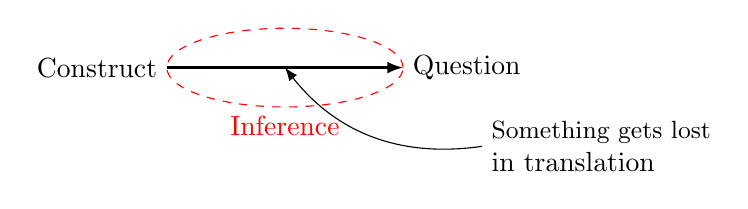
\begin{tikzpicture}[scale=1]
\node [left] at (0,0) {Construct};
\draw [-{Latex[length=2mm]}, thick] (0,0) -- (3,0);
\node [right] at (3,0) {Question}; \pause
\draw [red,dashed] (1.5,0) ellipse (1.5 and .5);
\node [align=center,below,red] at (1.5,-.5) {Inference};\pause
\node [align=left, right]  at (4,-1) {\small Something gets lost\\in translation};
\path [-Latex] (4,-1) edge [bend left=30] (1.5,0) {};
\end{tikzpicture}
\end{center}
\end{frame}

\begin{concept}{validity}
{The accuracy with which our measures reflect the true underlying value}
\end{concept}

\begin{frame}{}
\begin{center}
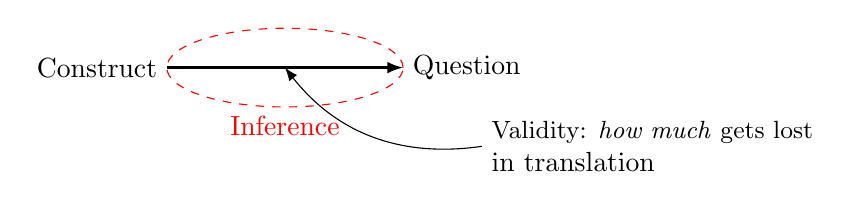
\begin{tikzpicture}[scale=1]
\node [left] at (0,0) {Construct};
\draw [-{Latex[length=2mm]}, thick] (0,0) -- (3,0);
\node [right] at (3,0) {Question};
\node [align=left, right]  at (4,-1) {\small Validity: \emph{how much} gets lost\\in translation};
\path [-Latex] (4,-1) edge [bend left=30] (1.5,0) {};
\draw [red,dashed] (1.5,0) ellipse (1.5 and .5);
\node [align=center,below,red] at (1.5,-.5) {Inference};
\end{tikzpicture}
\end{center}
\end{frame}

\begin{frame}{Psychometrics}
\centering
\[
\left.
\begin{array}{l}
\text{I ask you one question} \\
\text{I ask you five questions}
\end{array}\right\} \text{Which measures apptitude better?}
\]
\end{frame}

\begin{concept}{reliability}
{How closely repeated measurements of the same construct yield the same result}
\end{concept}

\begin{frame}{Validity \& Reliability}
\begin{center}
\begin{tabular}{rp{3in}}
\textbf{reliability} & degree to which measurement of the same construct yields the same answer over repeated trials \emph{with the same person}\\[.5em]
\textbf{validity} & degree to which the measure accurately represents the underlying construct
\end{tabular}
\end{center}
\end{frame}

\begin{frame}
\textbf{\textsc{It is really, really important that measurement error should not be biased!!!}}
\end{frame}

\section{Representational Inference}

\begin{frame}{Representational Inference}
\begin{center}
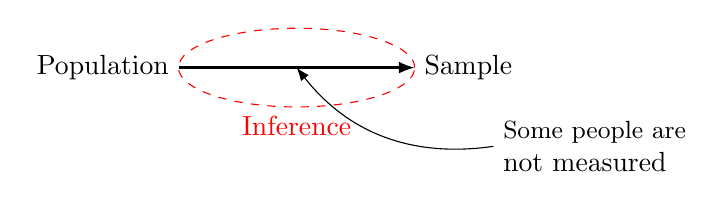
\begin{tikzpicture}[scale=1]
\node [left] at (0,0) {Population};
\draw [-{Latex[length=2mm]}, thick] (0,0) -- (3,0);
\node [right] at (3,0) {Sample};
\node [align=left, right]  at (4,-1) {\small Some people are\\ not measured};
\path [-Latex] (4,-1) edge [bend left=30] (1.5,0) {};
\draw [red,dashed] (1.5,0) ellipse (1.5 and .5);
\node [align=center,below,red] at (1.5,-.5) {Inference};
\end{tikzpicture}
\end{center}
\end{frame}

\begin{frame}
\begin{figure}[h!]
\begin{center}
\includegraphics[height=7cm]{../images/GrovesCh2Fig2.pdf}
\end{center}
\end{figure}
\end{frame}


\end{document}


